\chapter{Investment as a hyperbolic rotation}
\label{chap:finance}

\section{Terminology}
The aim of this research is to refine the way that economic engineering currently deals with financial instruments, primarily fixed-interest assets, but also marketable equity (stocks), derivatives et cetera. All of these can be regarded as `investments', for lack of a better word, because they require a \emph{principal}, that is the amount investment, and a certain return that is proportional to the principal. This is why the return is usually expressed as a percentage of the principal, which in the case of debt is the interest rate. The later contains the word `rate', because it has an inherent timely aspect: interest rates (and returns of investments in general) are associated with a certain `term' or duration over which the return is realized. As such, any type of investment is characterized by three components:
\begin{itemize}
    \item a \emph{principal}, something that is originally invested;
    \item a \emph{return} proportional to the principal;
    \item a \emph{period} over which the return is realized.
\end{itemize}
In the world of finance, the principal and return often refer to some amount of money, but that does not necessarily have to be the case. For example, some stocks pay \emph{stock dividends}, which means that dividends take the form of additional stock. Alternatively, one could look outside finance to other factors of production, such as land: a farmer may `invest' a certain amount of land to gain the earnings (crops that grow on it) after the period of one year; of course, the amount of crops grown is proportional to the surface area of the land that the farmer has cultivated.

\section{Reinvestment of earnings}
After the end of the investment period, the investor has two options: either he can spend his earnings, or he can reinvest them; essentially, he starts the next investment period with a higher principal than the first one. This reinvestment of capital is a crucial concept in the world of finance and is the reason for the existence of compound interest. Indeed, compound interest assumes that ones earnings after one period also bear interest; the so-called \emph{interest on interest}. This can be illustrated by means of the example shown in \cref{fig:compound_interest}. An investor holds a fixed-interest investment with a principal of \$1000 and an interest rate of 5\% annually. After one compounding period, he naturally earns \$50 directly on the principal. As such, his direct earnings, which will be called `yield', now amount to \$50 while the invested `capital' is still \$1000. The next compounding period however, provided that the investor does not withdraw his earnings from the account, the \$50 generate \$2.5 of interest as well, which are \emph{reinvested}; i.e. they take the form of capital instead of yield. Simultaneously, the investor als keeps the additional benefits from the \$1000 of capital in the form of another \$50 dollars of direct earnings.
\begin{figure}[h]
    \centering
    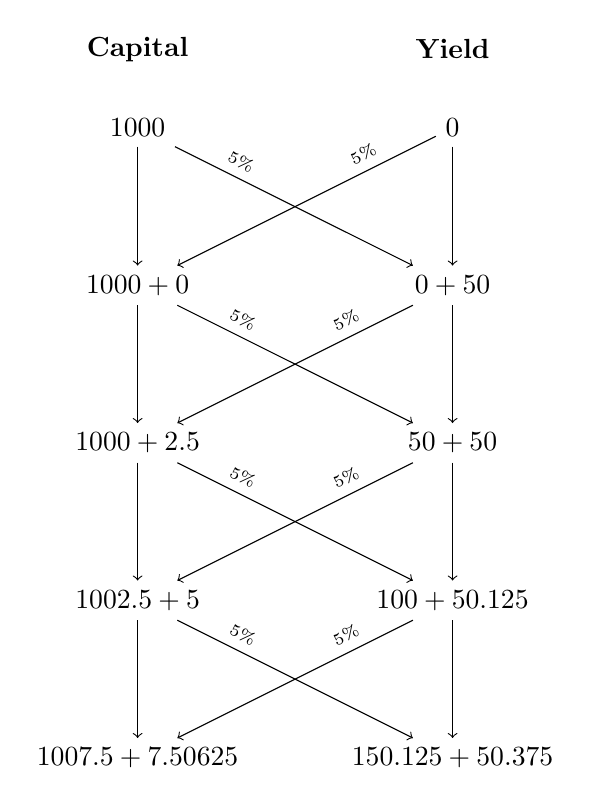
\begin{tikzpicture}
    \path (-2, 1)  node[fill=white, align=center]     {\textbf{Capital}};
    \path (2, 1)   node[fill=white, align=center]     {\textbf{Yield}};
    \path (-2, 0)  node[fill=white, align=center](x1) {1000};
    \path (2, 0)   node[fill=white, align=center](y1) {0};
    \path (-2, -2) node[fill=white, align=center](x2) {\(1000 + 0\)};
    \path (2, -2)  node[fill=white, align=center](y2) {\(0 + 50\)};
    \path (-2, -4) node[fill=white, align=center](x3) {\(1000 + 2.5\)};
    \path (2, -4)  node[fill=white, align=center](y3) {\(50 + 50\)};
    \path (-2, -6) node[fill=white, align=center](x4) {\(1002.5 + 5\)};
    \path (2, -6)  node[fill=white, align=center](y4) {\(100 + 50.125\)};
    \path (-2, -8) node[fill=white, align=center](x5) {\(1007.5 + 7.50625\)};
    \path (2, -8)  node[fill=white, align=center](y5) {\(150.125 + 50.375\)};
    
    \draw[->] (x1) -- (x2);
    \draw[->] (x2) -- (x3);
    \draw[->] (x3) -- (x4);
    \draw[->] (x4) -- (x5);
    
    \draw[->] (y1) -- (y2);
    \draw[->] (y2) -- (y3);
    \draw[->] (y3) -- (y4);
    \draw[->] (y4) -- (y5);
    
    \draw[->] (x1) -- node[near start, sloped, above] {\footnotesize{\(_{5\%}\)}} (y2);
    \draw[->] (x2) -- node[near start, sloped, above] {\footnotesize{\(_{5\%}\)}} (y3);
    \draw[->] (x3) -- node[near start, sloped, above] {\footnotesize{\(_{5\%}\)}} (y4);
    \draw[->] (x4) -- node[near start, sloped, above] {\footnotesize{\(_{5\%}\)}} (y5);
    \draw[->] (y1) -- node[near start, sloped, above] {\footnotesize{\(_{5\%}\)}} (x2);
    \draw[->] (y2) -- node[near start, sloped, above] {\footnotesize{\(_{5\%}\)}} (x3);
    \draw[->] (y3) -- node[near start, sloped, above] {\footnotesize{\(_{5\%}\)}} (x4);
    \draw[->] (y4) -- node[near start, sloped, above] {\footnotesize{\(_{5\%}\)}} (x5);
\end{tikzpicture}

    \caption{A simple example of compound interest with a principal of \$1000 and an interest of 5\%. The direct earnings on the capital are called `yield', while the (re)invested amount is called `capital'.}
    \label{fig:compound_interest}
\end{figure}
This reinvestment of earnings is the driving force behind compound interest: without this step the investor would end up with \emph{simple interest}, which sees its relative returns essentially decreasing over time. One should, however, be cautious to associate this process exclusively with financial investments; for example a farmer could use the earnings from his land to buy more land, increase his earnings, use those again to buy even more land and so forth --- this will again give rise to a exponential growth. The farming example makes it quite clear that the object that `generates' the return (capital) is of a very different nature than the return itself (yield). They can be connected through the usage money as both a unit of account and a medium of exchange, which makes the whole process work \cite{Mankiw2017}. 

Financial investments are arguably the culmination of this concept, since money itself earns money that can be reinvested again instantaneously. Still, the capital-yield distinction remains relevant: for example, companies pay dividends to their shareholders in proportion to the amount of stock they own; the shareholders could then choose to reinvest these earnings in more stock of that (or another) company, increasing their `capital'. An additional example here are stock dividends, which are stocks with dividends that are paid as additional stock --- essentially taking the role of money out of the equation.

\section{The hyperbolic shape of compound interest}
If the numbers from the example in \cref{fig:compound_interest} are plotted against each other, with capital on the horizontal axis and yield on the vertical axis, a hyperbolic shape appears, shown in \cref{fig:hyperbolic_compounding}. Hyperbola are characterized by the implicit equation 
$$ X^2 - Y^2 = K^2, $$
where \lsymb{$K$}{Original investment} represents the `radius' of the hyperbola, which coincides with the principal amount of the investment. The amount of capital and yield accumulated at a certain time are then on the \lsymb{$X$}{Capital} and \lsymb{$Y$}{Yield}-axis respectively. However, as \cref{fig:hyperbolic_compounding} demonstrates, the shape arising from the example is not quite hyperbolic, since it essentially lags behind the real hyperbola of that radius.
\begin{figure}[h!]
    \centering
    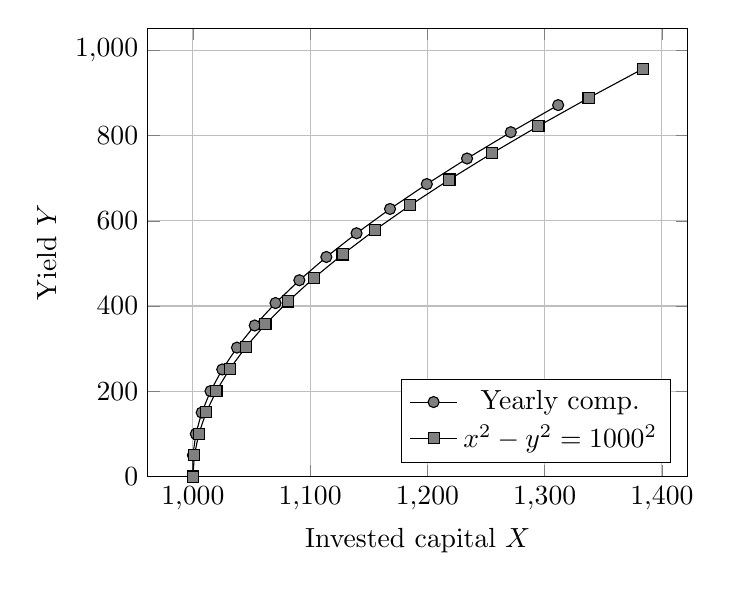
\begin{tikzpicture}[scale=1]
    \begin{axis}[
        xlabel={Invested capital $X$},
        ylabel={Yield $Y$},
        grid,
        cycle list name= black white,
        legend pos = south east,
        ymin = 0,
    ]
        \addplot coordinates {
                    (1000   ,  0     )
                    (1000   ,  50     )
                    (1002.5,  100    )
                    (1007.5,  150.125)
                    (1015.01,  200.5 )
                    (1025.03,  251.25)
                    (1037.59,  302.502)
                    (1052.72,  354.382)
                    (1070.44,  407.018)
                    (1090.79,  460.539)
                    (1113.82,  515.079)
                    (1139.57,  570.77)
                    (1168.11,  627.748)
                    (1199.5,  686.154)
                    (1233.8,  746.128)
                    (1271.11,  807.818)
                    (1311.5,  871.374)
                    % (135.507,  93.6949)
                    % (140.192,  100.47)
                    % (145.215,  107.48)
        };
        \addlegendentry{Yearly comp.};
        
        \addplot coordinates {
            (1000., 0.0)
            (1001.2502604383691, 50.020835937655015)
            (1005.0041680558036, 100.16675001984403)
            (1011.2711095766704, 150.56313315161269)
            (1020.0667556190758, 201.336002541094)
            (1031.4130998795731, 252.6123168081683)
            (1045.3385141288605, 304.52029344714266)
            (1061.8778191559855, 357.18972943727195)
            (1081.0723718384547, 410.7523258028155)
            (1102.970168555971, 465.34201693419774)
            (1127.6259652063807, 521.0953054937474)
            (1155.101414123941, 578.1516037434543)
            (1185.4652182422679, 636.6535821482414)
            (1218.793302887456, 696.7475261264401)
            (1255.169005630943, 758.5837018395335)
            (1294.6832846768447, 822.3167319358299)
            (1337.4349463048446, 888.1059821876231)
            (1383.530891937359, 956.1159599886322)
            %(143.30863854487743, 102.65167257081754)
            %(148.62253413851738, 109.94843179306726)
            %(154.30806348152436, 117.52011936438014)
        };
        \addlegendentry{$x^2 - y^2 = 1000^2$};
        
    \end{axis}
\end{tikzpicture}

    \caption{Plot of the numbers from the example }
    \label{fig:hyperbolic_compounding}
\end{figure}
The reason why the `perfect' hyperbola is not recovered in the example is demonstrated as follows. The capital-yield evolution can be modeled as a second-dimensional difference equation like so:
$$ \mqty(X(k+1)\\Y(k+1)) = \mqty(1& r \\ r & 1)\mqty(X(k)\\Y(k))\qq{with }X(0) = K,\, Y(0) = 0 $$
where $X$ denotes capital, $Y$ denotes yield and $r$ is the interest rate. The solution of this autonomous system is given by:
$$ \mqty(X(k)\\Y(k)) = \mqty(1& r \\ r & 1)^k\mqty(\ininv\\0). $$
One can then write $X(k)^2 - Y(k)^2$ in terms of this solution:
$$ X(k)^2 - Y(k)^2 = \mqty(K & 0)\mqty(1& r \\ r & 1)^k\mqty(1 & 0\\0 & -1)\mqty(1& r \\ r & 1)^k\mqty(K\\0).$$
In order to easily evaluate the matrix powers, one can use the eigenvalue decomposition:
with
$$ \mqty(1 & r \\  r & 1)^k = V\Lambda^k V^{-1} \qq{with } V = \mqty(-1 & 1 \\ 1 & 1) \quad \Lambda = \mqty(1 - r & 0\\0 & 1 + r). $$
Straightforward computations then yield:
$$ X(k)^2 - Y(k)^2 = K^2\qty(1 - r^2)^k, $$
which suggests that for reasonably small values of $r$, the compounding process approximates the equation for the hyperbola. One way to achieve this is to compound faster, i.e. to use more periods with a smaller interest, such that $r \mapsto r/n$ and $k \mapsto kn$ for $n \to \infty$. Indeed, 
$$ \lim_{n\to\infty} K^2\qty(1 - \qty(\frac{r}{n})^2)^{kn} = K^2. $$
That is, for infinitely fast compounding, the capital-yield decomposition of compound interest follows a hyperbolic shape.

Another way to view this is to see the difference equation as a sampled version of an underlying continuous system. One can find the continous-time state-transition matrix by applying the matrix logarithm to its discrete-time counterpart:
    $$ \log \mqty(1 & r \\ r & 1) = 
        \frac{1}{2}\mqty(\log(r + 1) + \log(r - 1) & \log(r + 1) - \log(r - 1)\\
                         \log(r + 1) - \log(r - 1) & \log(r + 1) + \log(r - 1)). $$
This continuous-time state-transition matrix has eigenvalues $\log(1 + r)$ and $\log(1 - r)$, the former of which is the continuous-time equivalent interest rate, or the \emph{force of interest}, $r_c$ \cite{Kellison1991}. From this discussion, one can infer that the disrcrete compounding process is essentially an approximation of the underlying `ideal' continuous-time process, which is why the rotational analogy will be developed for a continuous compounding scenario; since the discrete-time equivalent may always be obtained by means of sampling.

\section{The rotational analogy}


